\documentclass[12pt]{ctexart}
\usepackage{graphicx}%图片引用包
\usepackage{amssymb}%特殊符号
\usepackage{amsmath,amsfonts,bm}%矩阵
\usepackage{amsthm}%定理
\usepackage{geometry}%缩放
\usepackage{hyperref}%超链接
\usepackage{cite}
\usepackage{framed}%框框
\usepackage{color}%颜色
\usepackage{mathrsfs}%花体
\usepackage{anyfontsize}
\usepackage{indentfirst}%缩进
\usepackage{extsizes}%size
\usepackage{newtxtext,newtxmath}%times风格字体
\usepackage{mdframed}%边栏
\usepackage{enumerate}
\usepackage{braket}
\usepackage{footnote}
\usepackage{etoolbox}
\usepackage{url}


\BeforeBeginEnvironment{framed}{\savenotes}
\AfterEndEnvironment{framed}{\spewnotes}
\surroundwithmdframed[
  linecolor=gray,
  topline=false,
  bottomline=false,
  rightline=false,
  linewidth=4pt,
  innerleftmargin=10pt,
  innerrightmargin=10pt,
  innertopmargin=0pt,
  innerbottommargin=5pt
]{theorem}
\surroundwithmdframed[
    linecolor=black,
    leftline=false,
    rightline=false,
    linewidth=0.5pt,
    innerleftmargin=10pt,
    innerrightmargin=10pt,
    innertopmargin=0pt,
    innerbottommargin=5pt
]{note}

\newtheorem{theorem}{Theorem}
\newtheorem{note}{Note}
\geometry{a4paper,scale=0.85}
\hypersetup
    {
        hypertex=true,
        colorlinks=true,
        linkcolor=blue,
        anchorcolor=blue,
        citecolor=blue
    }


\title{Basis of Single Molecular Localization Microscopy\\单分子定位超分辨成像技术基础}

\author{Jerry Ling} 

\date{\today}
 
\begin{document}  %begin后括号内是文件类型
\maketitle  %生成标题
相较于普通的衍射受限(diffraction limited, 指受到衍射极限制约)的显微镜,SMLM是一类大幅提升空间分辨率、能够在分子尺度上对精细生物结构成像的技术\footnote{其发展历史可见末页Notes,亦可参考章效锋《显微传》。}。通过计算或拟合(如对光斑进行高斯拟合),SMLM能够以较高的精度对\textbf{多张}衍射受限的图像中的\textbf{单个}发光分子进行定位(locolize),进而由这些定位(locolizations)生成超分辨率(20-50nm)的图像或分子运动轨迹(trajectories)。其中,特殊设计的、具有闪烁性质、分外明亮的、或具有各类靶向性的荧光染料为之提供了分子基础。为了明晰其中基本逻辑,本笔记将主要基于综述文献\cite{lelekSinglemoleculeLocalizationMicroscopy2021},逐一细察荧光染料及亮暗态切换原理、标记策略、设备搭建和数据和分辨率分析,并提供一些和本组研究相关的参考(感谢张老师的批注指正)。

\begin{figure}[t] %two figures
    \centering
    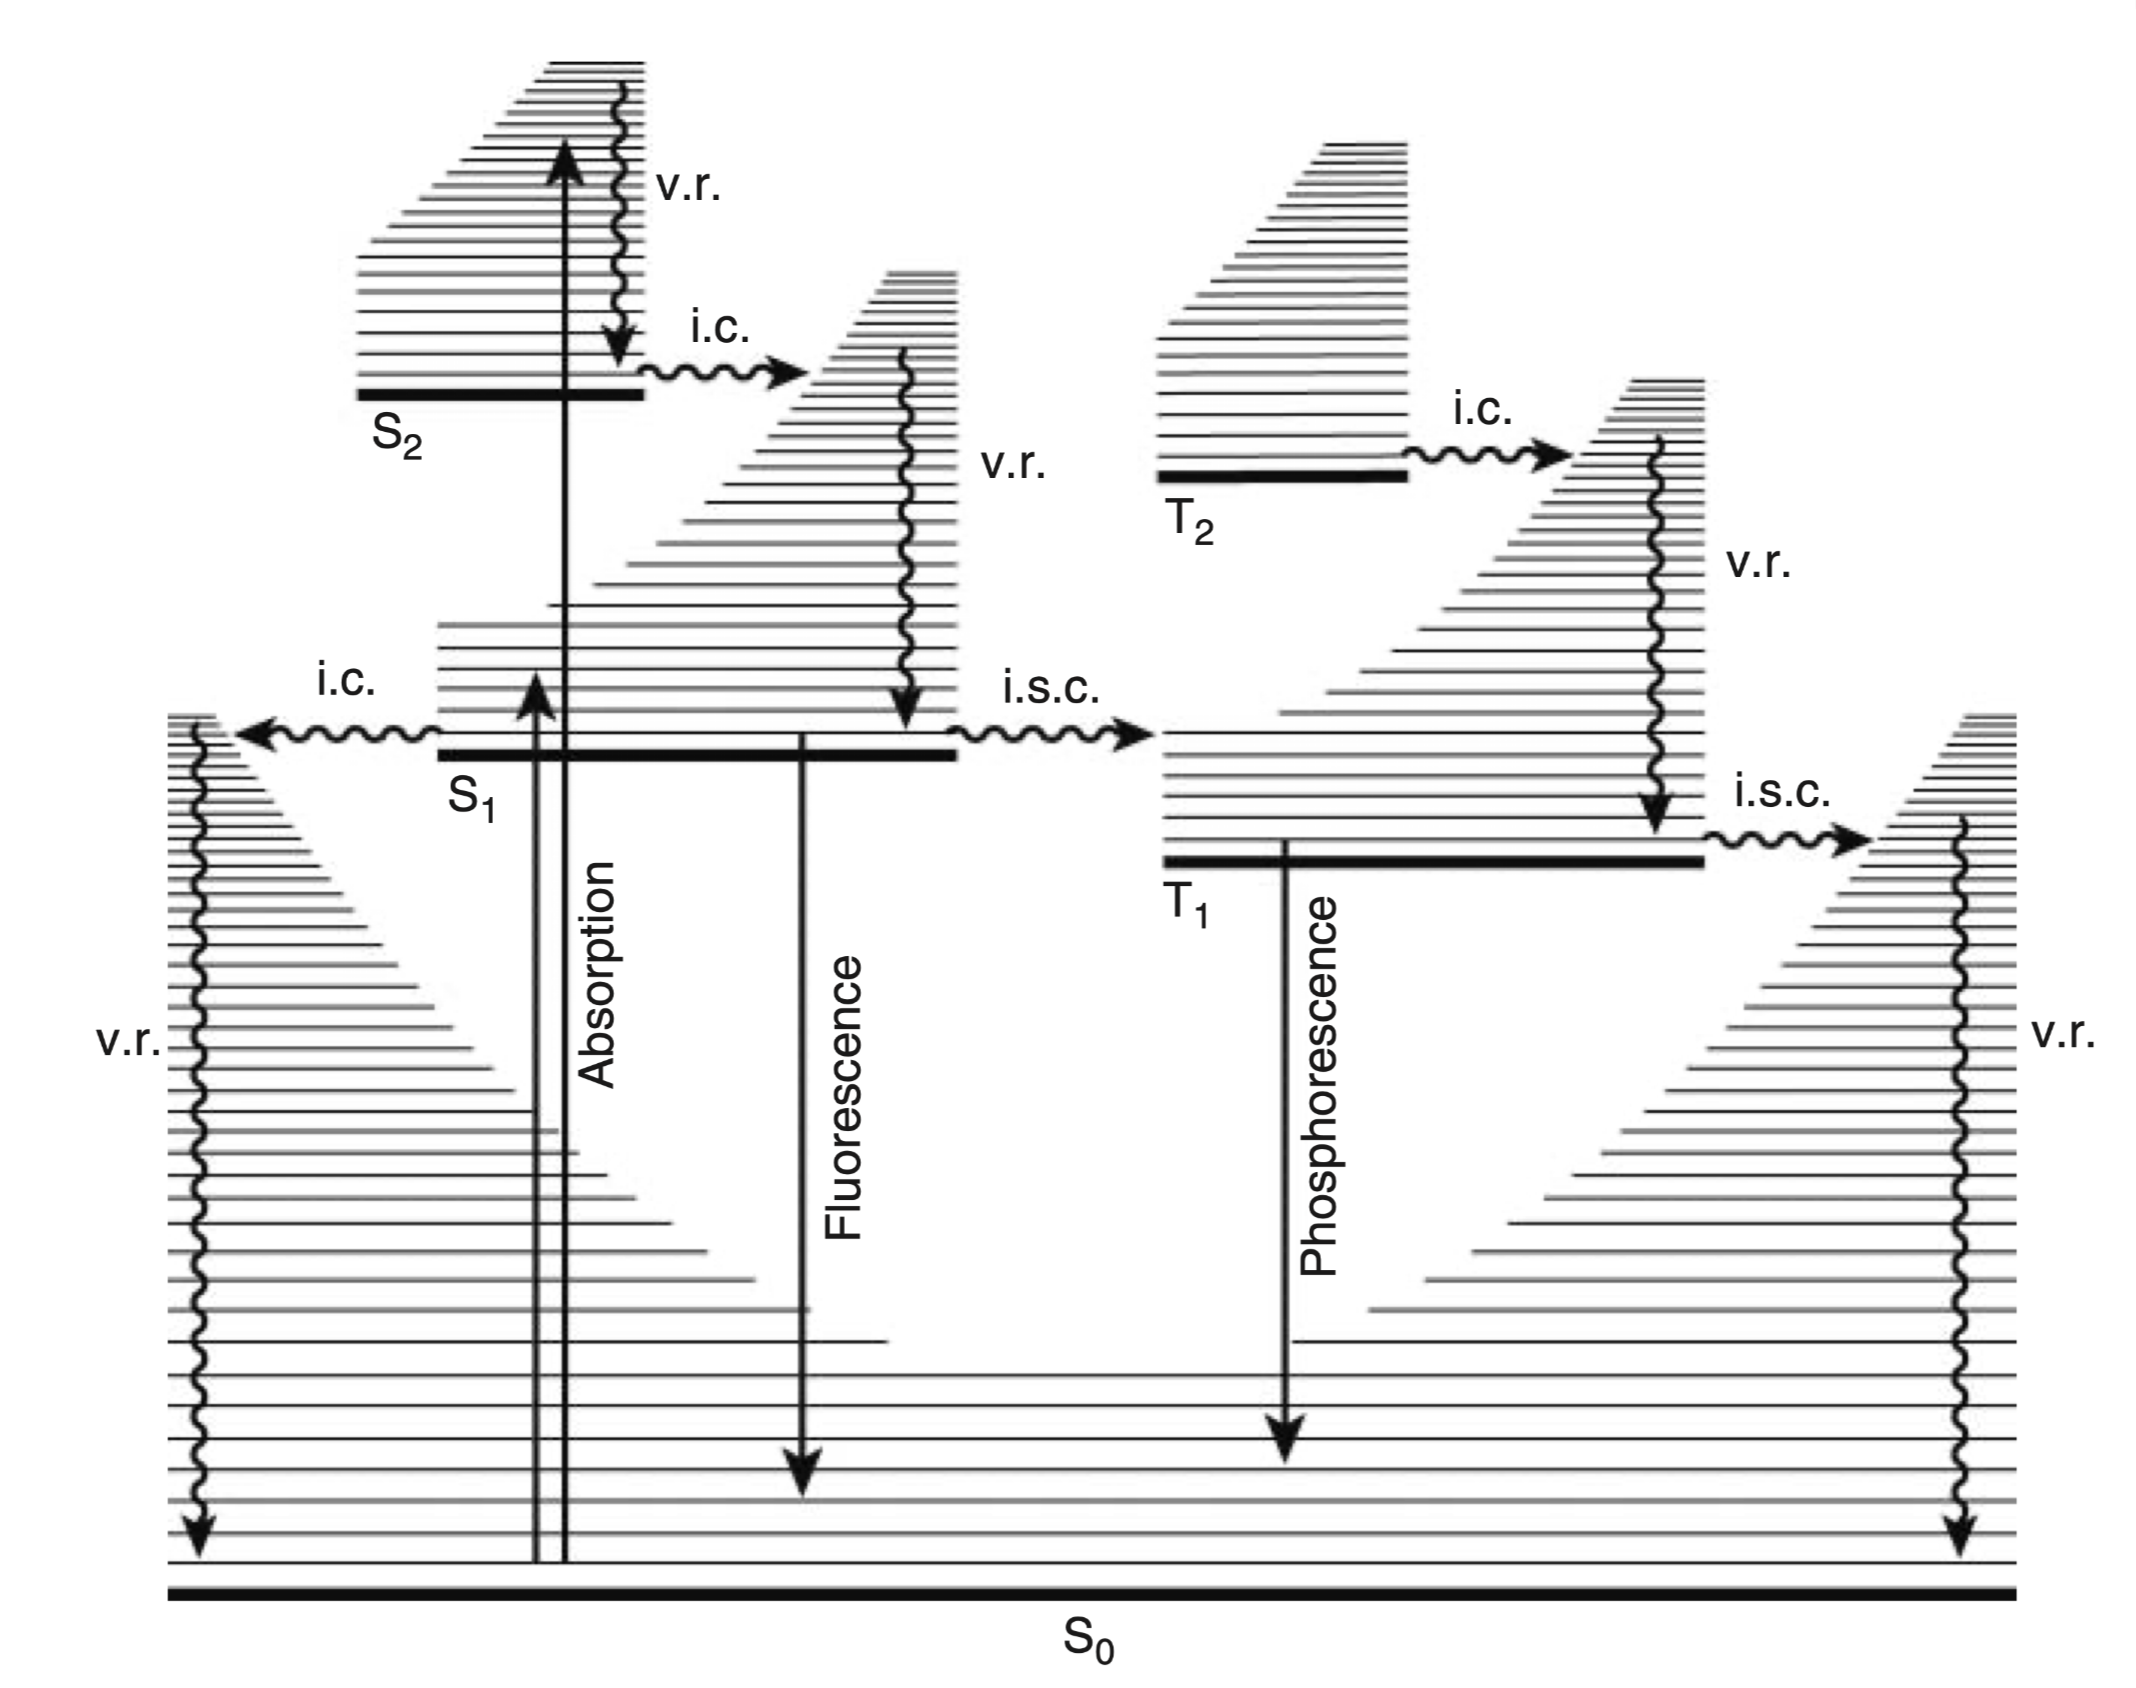
\includegraphics[width=0.6\textwidth]{Kinetic_diagram}
    \caption{Kinetic Diagram of Molecular Fluorescence}
    \label{Kinetic}
\end{figure}
\section*{开关:光反应的控制艺术}
根据超分辨成像的需求,考虑能够在\textbf{亮态(ON)}和\textbf{暗态(OFF/dark state))}间转化的荧光分子:
\begin{framed}
    \begin{enumerate}[a)]
        \item 在两态间可逆转换(存在平衡),即自发闪烁\footnote{我们发展了自发闪烁的近红外染料(陈松:\href{https://pubs.acs.org/doi/abs/10.1021/acs.analchem.4c02445}{pH响应罗丹明+步花青};炳捷:\href{https://pubs.acs.org/doi/10.1021/acs.nanolett.4c00595}{自发闪烁方酸})还将自发闪烁SiRhod用于\href{https://pubs.acs.org/doi/10.1021/cbmi.5c00037}{膨胀显微}(杨璐)。我们还发现了UCNP的自发闪烁现象。(佳玲/茂江:Ho-UCNP/SPUM) --YZ}
        \item 原本不发光,通过激光(UV)部分激活,在最大吸收光作用下发生光漂白(PALM)\footnote{PALM最早都是用可光激活荧光蛋白实现的。一般激活光是UV或者紫等高能光子,后来我们发展了可见光激活的染料。(见学博的工作[\href{https://onlinelibrary.wiley.com/doi/abs/10.1002/ange.202211767}{Universal Photoactivatable Tag}]和金阳的工作[\href{https://pubs.acs.org/doi/10.1021/acsnano.5c03182}{RELAST}]) --YZ}
        \item 原本可发荧光,在最大吸收光作用下生成长时间稳定的暗态,且能通过激光(UV/活化分子传递)激活至亮态(STROM)
    \end{enumerate}
\end{framed}
\noindent 其中态间的转化的光物理/光化学过程决定了其特性和调控的方式。下面简要回顾荧光的基本过程:
\subsection*{荧光基本过程和概念}
\par 分子的荧光过程可参考图\ref{Kinetic}示意。基态($S_0$)的电子在激发光作用下发生跃迁,进入激发态($S_1$)的某振动能级上(Frank-Condon原理)。其跃迁速率可通过微扰理论导出:
\begin{equation}
    \omega(if)=\omega(fi)\propto \rho(\mu_{if})\bra{i}\hat{\mu}\ket{f}^2
    \label{pert}
\end{equation}
其中i和f表示始、终态,$\rho$指对应能级差的\textbf{辐射密度},$\bra{i}\hat{\mu}\ket{f}$是跃迁\textbf{矩阵元(transition moment)},两态间的算符是偶极矩算子。注意到两个方向的跃迁几率一致,分别称为\textbf{受激吸收(induced absorption)}和\textbf{受激发射(induced emission)}。后者与激发光同相同向,对我们而言不重要。该过程使能级布局数偏离统计平衡态,被激发的电子需要以某种方式返回平衡态:
\begin{itemize}
    \item 振动弛豫(vibrational relaxation, v.r.):非辐射过程,很快,使得激发到S1振动能级上的电子快速返回S1振动基态
    \item 内转换(internal conversion, i.c.):非辐射过程,自旋不变转换至电子基态的高振动能级上,而后立刻进入振动弛豫
    \item \textbf{自发辐射(spontaneous emission)}:各向同性的发光,由图可见其波长一般大于吸收光,即通常意义上的\textbf{荧光(fluorescence)}。
    \item \textbf{系间穿越(intersystem crossing, i.s.c.)}:由单线态向附近三线态转移的非辐射过程。通常自旋禁阻,但在有机染料分子中常见(n,$\pi^*有轨道存在$)。这步过程是不少有机染料闪烁的重要步骤。若三线态辐射跃迁回基态,所发出的光一般称为磷光,寿命通常大大高于荧光($10^{-4}s$ v.s $10^{-7}s)$。
\end{itemize}
在我们的问题中,染料(如Cy5)具有较大的系间穿越速率。而在体系中加入巯基等还原剂($\beta$-ME)能进一步形成稳定的加合物,即出现长时间的\textbf{暗态}(寿命可长达数秒)。然而其中涉及复杂的光物理和光化学过程(如单光子参与的光电子传递反应,photoelectron transfer),其机理尚待更多研究阐明。
\par 除了上述光物理过程和还原剂参与反应外,处理荧光分子还另需考虑\textbf{光漂白(photobleaching,不可逆光反应)}的问题。如体系中的氧气是常见的导致光漂白的物质,在需要的情况下必须进行除氧处理。
\begin{note}[lifetime explaned]
    处理荧光染料特性时候各种寿命容易混淆,特此说明较重要的几种参数:
    \begin{itemize}
        \item 荧光寿命 (fluorescence lifetime):指$S_1$态的寿命,因为对环境的敏感性常用于荧光寿命成像(见本目录另一篇note)。实验上通过脉冲激发后测量时间分辨的光子数获得指数衰减的曲线拟合得到:\[\tau=\frac{1}{k_{F}+k_{ST}+k_{relax}}\]
        \item 亮态寿命 ($\tau_b$ or $\tau_{ON}$):指在持续激发下亮态的寿命,可能是光漂白或暗态转化所致。与荧光寿命不同的是,亮态寿命通常和\textbf{激发光强度}有关,因为其反应通常涉及光子。
        \item 暗态寿命 ($\tau_d$ or $\tau_{OFF}$):概念同亮态相似。测量亮暗态寿命可以直接记录荧光强度进行指数拟合,也可进行单分子“轨迹”分析,见下节。
    \end{itemize}
    P.S.(荧光寿命光强无依赖性)由式(\ref{pert})可看出,激光强度影响仅激发几率,也即影响能级布居(population)。布居数增加则会间接影响荧光\textbf{发射强度},但不影响荧光寿命,因为光子不参与自发辐射过程(若光强足够大则属于非线性光学,需另作考虑):
    \[I_{f}=N_{S_1}k_{F}\]
\end{note}


\subsection*{常用的开关分子及其典型信号}
\begin{figure}[b] %two figures
    \centering
    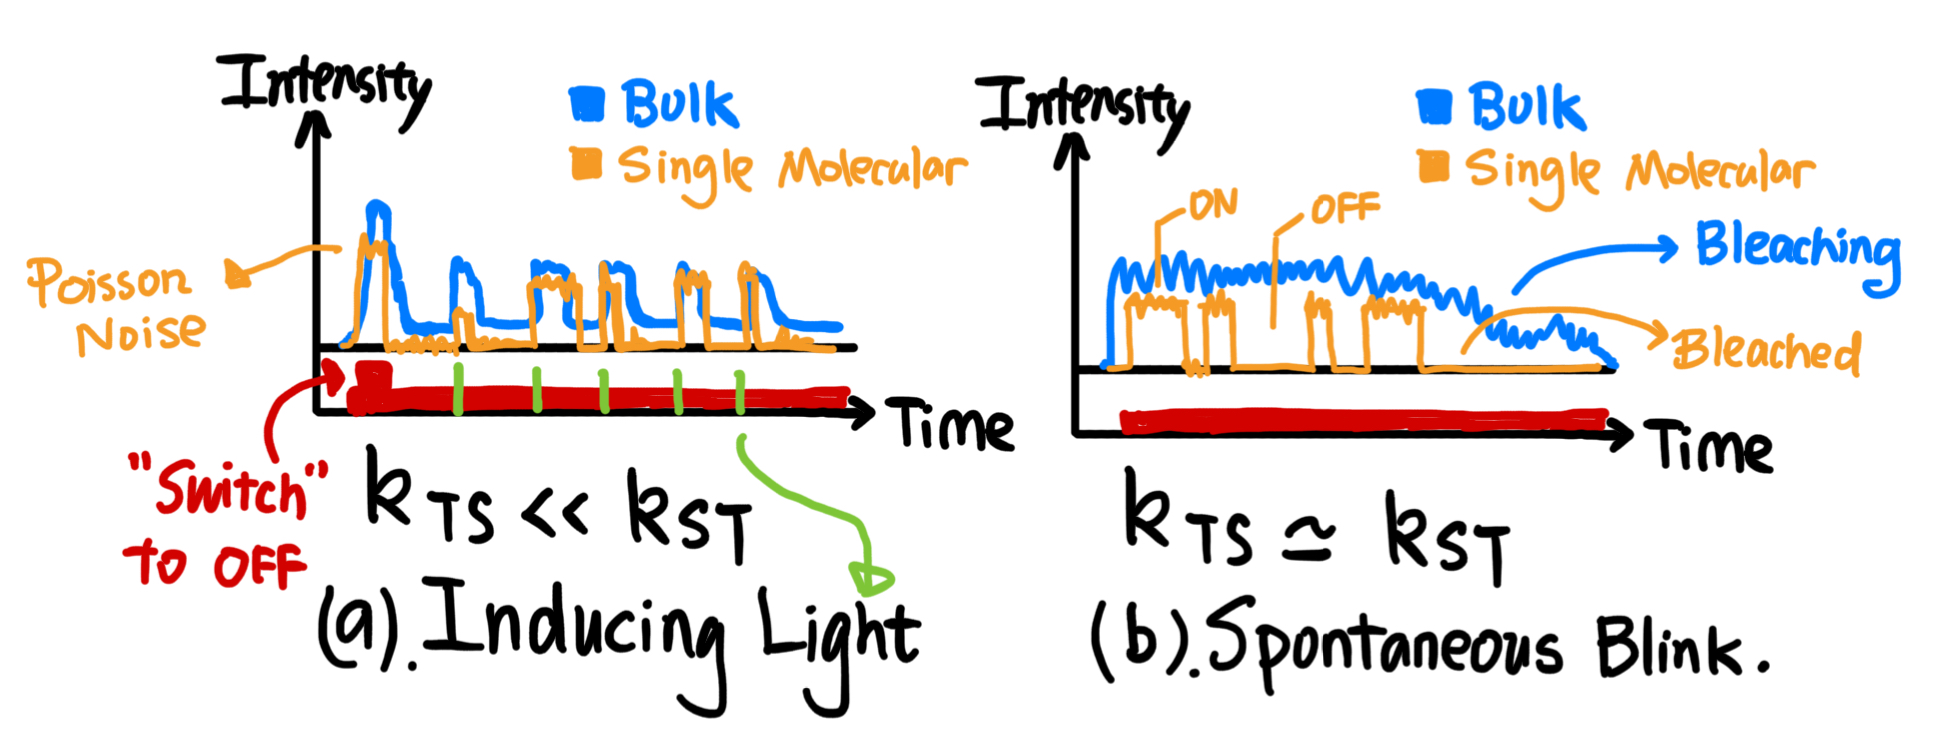
\includegraphics[width=0.8\textwidth]{Dynamic_diagram.jpeg}
    \caption{Intensity of Bulk and Single Molecule w.r.t. Time}
    \label{Dynamic}
\end{figure}
在显微镜下,我们有研究单分子发射信号的能力。考察每一个单分子的状态,则不难发现其反应的过程是一个基于一定参数的随机过程。若体系宏观上是均匀的,那么对单分子行为进行统计就能获得一个无偏的宏观动力学估计器。下面对常用的荧光分子进行介绍,并给出其典型的单分子和整体信号(见图\ref{Dynamic})。
\begin{enumerate}[i)]
    \item 光开关(photoswitchable):Cy5,Alexa Fluor 647;Alexa Fluor dyes,ATTO dye。典型条件10-200mM $\beta$-ME + enzymatic oxygen scavenger。控制氧气-还原剂\textbf{含量}和\textbf{激发光强度}可以控制亮态(5-20ms)暗态(seconds)寿命。暗态到亮态到激活可用紫外(405nm)或邻近的激发分子(Cy3)。每次控制激发的数量以保证不重叠并减少光漂白是成功成像的关键。
    \item 光激活(photoactivatable):photochromic rhodamine amides30, Janelia Fluor® 549, PA Janelia Fluor® 646,Cy5B。UV激活,但在下一次激活前需要用较长波长光漂白。荧光蛋白有PAmCherry\footnote{小写的m代表单体荧光蛋白:monomeric fluorescent protein。},PA-TagRFP,PA-GFP等。亮态被淬灭前的光子数决定了单帧定位精度,但较长的寿命也降低了帧率。
    \item 光转换(photoconvertiable):Eos,Dendra2,mMaple。紫外光可令其荧光颜色转化(Eos:488-561nm),如同光激活染料,需要漂白掉转化的分子后再进行下一次转化。
    \item 自发闪烁(selfblinking):HMSiR39,HEtetTFER40,RD。其闪烁源于化学反应而同激发强度无关,常通过pH调节其速率,可用于live cell成像。
\end{enumerate}
注意图\ref{Dynamic}每个周期中单分子进入暗态的时间是一个随机分布,而bulk中荧光衰减则是相同的。实验中暗态时可用较弱的激发光来“关闭”进入亮态的分子。“T”代表暗态,可能是三线态加合物,也可能是其他不发光的产物。
\section*{分辨率:标记、激发、光子数}
由于流程较长,超分辨成像的分辨率估计也较为复杂。首先,如果所有发射荧光的单分子都能精准定位,那么其分辨能力取决于\textbf{标记密度(labeling density)}。根据对一般采样定理的仔细分析(详见\cite{legantHighdensityThreedimensionalLocalization2016}),分辨频率最多达到标记密度的[5倍奈奎斯特频率],即为采样频率的五分之一(分辨率R单位m,频率$\nu$单位$m^{-1}$,间距$\Delta$单位m):
\begin{equation}
    R\leq R_{5*Nyq}\triangleq[\frac{\nu_{sample}}{5}]^{-1}=5\Delta_{sample} 
\end{equation}
譬如欲达到23nm的分辨率,则平均每4.6nm就应有一个标记分子被定位以达到该要求(P.S.标准\textbf{奈奎斯特频率}定义为采样频率的一半)。注意,合成图片的帧最好能将所有荧光分子locate至少一遍,或者located分子密度应当大于$R_{5*Nyq}$。
\par 其次,实际一定曝光时间的单分子不总是能准确、精确定位。若定位是无偏的,则一般认为分辨率还被其\textbf{精度(precision)}限制:
\begin{equation}\label{CRLB}
    R\geq R_{loc}\triangleq2.3\sigma_{loc}
\end{equation}
单分子发射的光子坐标(\textbf{点源扩散函数,PSF})本身应是一个近似的高斯分布的随机变量$N[(x,y),\sigma_0^2]$。我们实际上利用了N个样本(光子)在CMOS上的信号去估计该随机变量的坐标参数(x,y)。根据估计理论,估计器($\hat{x}$,$\hat{y}$)的方差必然大于其\textbf{MLE估计器}(最大似然估计)的方差:
\begin{theorem}[Cramér–Rao lower bound]
    \[Var(\hat{x})\geq-[\mathbb{E}\frac{\partial^2}{\partial x^2}\ln{p(L,x)}]^{-1}\]
\end{theorem}
其中p(L,x)指当\textbf{参数}为x时候观察到L的概率,也就是L取所有样本值时的联合概率密度分布。代入高斯分布,因为每个样本都是独立等同分布,可简化为:
\begin{equation}
    \sigma_{loc}\geq \frac{\sigma_0}{\sqrt{N}}
\end{equation}
注意,这个估计总是过于保守,且不考虑连接分子时导致的\textbf{偏差(bias)}。
\par 当取得了图像后,可以通过\textbf{傅立叶环相关分析(Fourier Ring Correlation)}估计分辨率。通过比较两张图在频域某半径为r的环内的相关性,得到图像在某一截止空间频率内的“稳定性”,以同时考虑精度和采样。而实验中最常用于展示分辨能力的方法是直接分辨\textbf{已知距离的生物结构}\footnote{若要估计分辨率,需要对一系列不同长度的已知结构进行分辨。 --YZ}。
\par 最后,当应用于\textbf{时间分辨}的成像如活细胞成像时,每张超分辨图像的重构帧数应当远小于生物动态的特征时间。实验上将所有帧分组(bining)或使用滑动窗口(sliding window)合成视频以实现动态成像\footnote{sliding window方法可保留更多动态细节,显著增加视频流畅。 --YZ}。
\section*{实验:标记、固定和光路搭建}
将荧光开关的基团/分子引入观测的对象是SMLM的第一步。\textbf{目标蛋白(target protein)}指希望标记上荧光基团的蛋白。不同标记方法也会引入不同的\textbf{连接误差(link error)}。可通过以下方法实现:
\begin{itemize}
    \item 编码荧光蛋白 Encoding fluorescent proteins:通过转染融合了荧光蛋白基因的目标蛋白基因来表达能发射荧光的目标蛋白。好的选择应减少荧光蛋白对目标蛋白功能的影响。
    \item 免疫标记 Immunolabelling:合成染料无法直接编码,需要先耦合到能够结合目标蛋白的抗体上,或耦合到能够连接到一抗的二抗上。后者能有较强的荧光强度,但也引入更大的连接误差。通常不适用于活细胞成像(需要穿透细胞膜)。
    \item 蛋白标签 Protein tag:为目标蛋白编码进特殊的基序(motif)以特异性地连接合成染料上的配体。具有最小的连接误差。
    \item 直接标记 Direct labelling:使用连接了染料的肽段或药物直接标记肌动蛋白或微管。尽管很小,但会降低生物活性而作为修饰剂。若染料修饰了脂类分子则可直接整合进生物结构中。基因编码\footnote{一个重要的标记方法是对蛋白表面伯胺(from Lys)用NHS染料进行标记,这种通常会每个蛋白标记\textbf{多个}染料;另一个常用的是定点引入表面半胱氨酸(Cys),当表面Cys个数大于等于2个时则定点突变以清楚多余Cys,然后用修饰了马来酰亚胺的染料标记,这种理想情况下一个蛋白标记一个染料分子。}允许引入非天然氨基酸,如能和TCO反应的赖氨酸,TCO-lys复合物和同生物正交试剂发生\textbf{点击反应(click reaction)}从而引入荧光染料。
\end{itemize}
\par 对于需要固定的细胞或组织,希望保持其结合位点和蛋白作用。\textbf{多聚甲醛PFA}和\textbf{戊二醛}是最常用的交联剂,\textbf{冰甲醇}或\textbf{乙二醇}可用于细胞骨架固定和形态学研究。30分钟的4\% PFA和0.2\%glutar-aldehyde处理可抑制膜流动性以避免团簇。免疫标记法需要在固定后\textbf{渗透化(permeabilize)},且需要在标记前加入BSA或NGS等blocking buffer以减少非特异性结合和背景噪音。此外,还可以用高压低温环境达到固定效果。而对于活细胞研究,细胞在PBS中被成像。\textbf{光毒性(Phototoxicity)}是需要考虑的因素,可用细胞分裂等方法测试之。
\par 成像只需要常用的传感器如EMCCD和sCMOS,后者敏感性较低但允许帧率更高,其像素大小应接近衍射极限(150-200nm)。光路方面使用二色镜可以分离、合并两种颜色的激光;灵活选择滤镜\footnote{滤镜可分为短通、长通、带通、notch等,可由透过率-波长图描述。目前光学间所有的滤镜及其透过率数据已录入数据库,需要者可以参考 \href{https://github.com/Jerry-LXH/FudanChemNotes/tree/main/SmilE/Optics_exp/Database_of_filters}{github仓库} ,不定期更新。}可滤除激发光而提高信噪比;仔细调整还可搭建\textbf{多通道}的系统\footnote{目前光学间常用双通道配置。需要注意的是双通道多色成像需要进行更仔细的数据处理(如dual color polynomial registration)以保证数据的可靠性。}。60–100x的油镜(N.A. > 1.4)\footnote{TIRF 物镜的NA通常大于1.45;尼康唯二的TIRFobj(60X/100X)的NA均为1.49. 目前光学间常用的即尼康的CFI Apochromat TIRF 100XC Oil油镜。}充当物镜以确保有效的光子收集。靠近盖玻片的样品可以使用\textbf{TIRF}来提升信噪比。使用特殊透镜调制信号可以实现\textbf{3d成像}。
\section*{数据处理和分析}
在SMLM中,每帧中亮起的分子应当在保证不重叠的条件下尽可能多,以尽快达到重构分辨率要求的帧数。开关分子的亮起由激光强度调控,且理论上可以使用反馈回路自动化,其曝光时间应接近ON-OFF的寿命(10-100ms)。用分辨率可以大致估计标记密度,用5-10倍的定位总数和每帧亮起的分子数估计总共需要的帧数,乘以曝光时间即总重构时间。
\par 时间分辨的结构动态成像方法见上文。跟踪单分子的方法则关注单分子的状态随时间的变化,称为\textbf{轨迹(trajectories)},以作为探针传递周围环境状态。此时标记密度不应过大以避免轨迹重叠,且应注意每帧曝光应选择使得单分子的位移大于定位精度\footnote{高通量\textbf{单分子追踪}和超分辨成像(死样本)还有前面提到的活细胞内细胞器\textbf{超分辨动态追踪}对成像参数都有不太一样的要求,此处暂不赘述,后文以超分辨成像的数据处理为例。}。SMLM使得其能够同时定位几倍于单分子方法的分子轨迹,以展示细胞中的分子动态(如扩散速率分布)。
\par SMLM的数据处理按单分子检测、单分子定位和超分辨图像重构进行,其中重点如下:
\begin{itemize}
    \item 检测:检测前首先要\textbf{去除背景},可用算法rolling ball ,difference of Gaussians,滤波器, 背景平均扣除。接着单分子信号可以用同PSF的互相关搜寻(correlation)。噪声可来源于:暗电流,读出噪声(极少),光电子放大器噪声,泊松噪声。
    \item 定位精度:按式(\ref{CRLB})估计最小精度,典型光子数在$10^2-10^4$,$\sigma_0\approxeq100$nm\footnote{红光波长较长,衍射光斑更大,可能较难达到100nm的精度。}。注意光学系统会导致PSF无法近似成高斯分布,背景噪声则会导致更差的精度。更好的精度估计公式参见:\textit{Kay, S. M. Fundamentals of Statistical Signal Processing Vol. 2: Detection Theory (Prentice Hall PTR, 1998).;Mortensen, K. I. el. Optimized localization analysis for single molecule tracking and super resolution microscopy. Nat. Methods 7, 377–381 (2010).}
    \item 定位算法:最大似然算法是所有算法的金标准,计算上通过迭代的梯度上升算法寻找最佳参数。PSF则常需要为每个实验单独标定以减少错误,更干净的背景能减少偏差。依靠图片处理单元,计算机现在已能够高效地完成这些任务。
    \item 后处理:可选择将邻近定位到的点合并为单个分子。另外,大部分SMLM实验需要进行\textbf{漂移矫正(drifting correction)},见后文。
    \item 重构:以上得到的坐标可以通过在亚像素(根据具体条件优化,一般在10-20nm)上显示来重构超分辨图像。每个点对应一定的像素亮度,经过线性叠加重构。
\end{itemize}
\par SMLM得到的数据可用于多种定量分析,如识别蛋白团簇、单分子计数、重建单个颗粒(需要该颗粒的多个相同成像)、多通道的共定位分析、单分子跟踪(Lagrangian/Eulerian)方法。常用的软件包(如ThunderSTORM)\footnote{目前已有很多基于机器学习的算法用于高密度数据的处理,可参见见\cite{hyunDevelopmentDeepLearningBasedSingleMolecule2022}}参见原始文献。

\begin{note}[the History of Single Molecular Localization Microscopy]
    单分子定位技术的历史比多数人想象的要早,此处简要列出其发展的时间线。(--provided by YZ)
    \begin{itemize} 
        \item 1940s: Cramér–Rao lower bound的数学理论建立,为SMLM提供了统计学基础。
        \item 1986: Norman Bobroff 将CRLB用于光度量学,说明了检测器上的点位置(the position of a spot)可以亚像素的精度估计。
        \item 1989: W.E. Moerner 和 L. Kador 首次以光学方法检测到单分子,证明了单分子的可观测性。
        \item 1996: T.H. Schmidt, G.J. Schütz, 与其同事首次报道了超越衍射极限的单荧光分子定位\textbf{实验}。
        \item Mid-1990s: 愈来愈多人将该理念用于单分子追踪(tracking)
        \item 2005: Paul Selvin 与其团队提出他们的FIONA技术,这是该理念在单分子追踪领域的专门应用。
        \item 2006: Eric Betzig (PALM)\cite{betzigImagingIntracellularFluorescent2006} 和 庄小威 (STORM)\cite{rustSubdiffractionlimitImagingStochastic2006} 同时提出将稀疏、随机激活的荧光分子引入SMLM中,首次真正实现了超分辨定位显微。
    \end{itemize}
\end{note}

\bibliography{/Users/jerryling/Documents/Research/Paper/MyLibrary}
\bibliographystyle{ieeetr}

\end{document}
